% This file was converted to LaTeX by Writer2LaTeX ver. 1.0
% see http://writer2latex.sourceforge.net for more info
\documentclass[twoside,letterpaper]{article}
\usepackage[latin1]{inputenc}
\usepackage[T1]{fontenc}
\usepackage[english]{babel}
\usepackage{amsmath}
\usepackage{amssymb,amsfonts,textcomp}
\usepackage{color}
\usepackage{array}
\usepackage{supertabular}
\usepackage{hhline}
\usepackage{hyperref}
\hypersetup{
    colorlinks,%
    citecolor=black,%
    filecolor=black,%
    linkcolor=black,%
    urlcolor=black
}

\usepackage{layout}
\usepackage{lscape}

\usepackage[pdftex]{graphicx}
\usepackage{picinpar}
\usepackage{wrapfig}
% Outline numbering
\setcounter{secnumdepth}{5}
\renewcommand\thesection{\arabic{section}}
\renewcommand\thesubsection{\arabic{section}.\arabic{subsection}}
\renewcommand\thesubsubsection{\arabic{section}.\arabic{subsection}.\arabic{subsubsection}}
\renewcommand\theparagraph{\arabic{section}.\arabic{subsection}.\arabic{subsubsection}.\arabic{paragraph}}
\renewcommand\thesubparagraph{\arabic{section}.\arabic{subsection}.\arabic{subsubsection}.\arabic{paragraph}.\arabic{subparagraph}}
\makeatletter
\newcommand\arraybslash{\let\\\@arraycr}
\makeatother
% List styles
\newcommand\liststyleWWviiiNumiii{%
\renewcommand\theenumi{\arabic{enumi}}
\renewcommand\theenumii{\arabic{enumii}}
\renewcommand\theenumiii{\arabic{enumiii}}
\renewcommand\theenumiv{\arabic{enumiv}}
\renewcommand\labelenumi{\theenumi)}
\renewcommand\labelenumii{\theenumii.}
\renewcommand\labelenumiii{\theenumiii.}
\renewcommand\labelenumiv{\theenumiv.}
}
\newcommand\liststyleWWviiiNumii{%
\renewcommand\theenumi{\arabic{enumi}}
\renewcommand\theenumii{\arabic{enumii}}
\renewcommand\theenumiii{\arabic{enumiii}}
\renewcommand\theenumiv{\arabic{enumiv}}
\renewcommand\labelenumi{\theenumi)}
\renewcommand\labelenumii{\theenumii.}
\renewcommand\labelenumiii{\theenumiii.}
\renewcommand\labelenumiv{\theenumiv.}
}
% Page layout (geometry)
\setlength\voffset{-1.4in}
\setlength\hoffset{-1in}
\setlength\topmargin{0.5in}
\setlength\oddsidemargin{1in}
\setlength\evensidemargin{1in}
\setlength\textheight{9in}
\setlength\textwidth{6.5in}
\setlength\footskip{0.561in}
\setlength\headheight{0.5in}
\setlength\headsep{0.461in}
% Footnote rule
\setlength{\skip\footins}{0.0469in}
\renewcommand\footnoterule{\vspace*{-0.0071in}\setlength\leftskip{0pt}\setlength\rightskip{0pt plus 1fil}\noindent{\rule{0.25\columnwidth}{0.0071in}}\vspace*{0.0398in}}
% Pages styles
\makeatletter
\newcommand\ps@Standard{
  \renewcommand\@oddhead
  \renewcommand\@evenhead{\@oddhead}
  \renewcommand\@oddfoot{{\textcolor{black}{\hfill SSDD Page }}\thepage}
  \renewcommand\@evenfoot{\@oddfoot}
  \renewcommand\thepage{\arabic{page}}
}
\makeatother
\setlength\tabcolsep{1mm}
\renewcommand\arraystretch{1.3}
\title{SYSTEM AND SOFTWARE ARCHITECTURAL AND DETAILED DESIGN DESCRIPTION}
\author{Paul Oman}
\date{2008-10-27}
\begin{document}
\begin{center}
SYSTEM AND SOFTWARE DESIGN DESCRIPTION (SSDD): Incorporating Architectural Views and Detailed Design Criteria \\
FOR \\
Groups in a University Setting
\\
Version 0.004 \\
December 2, 2010 \\

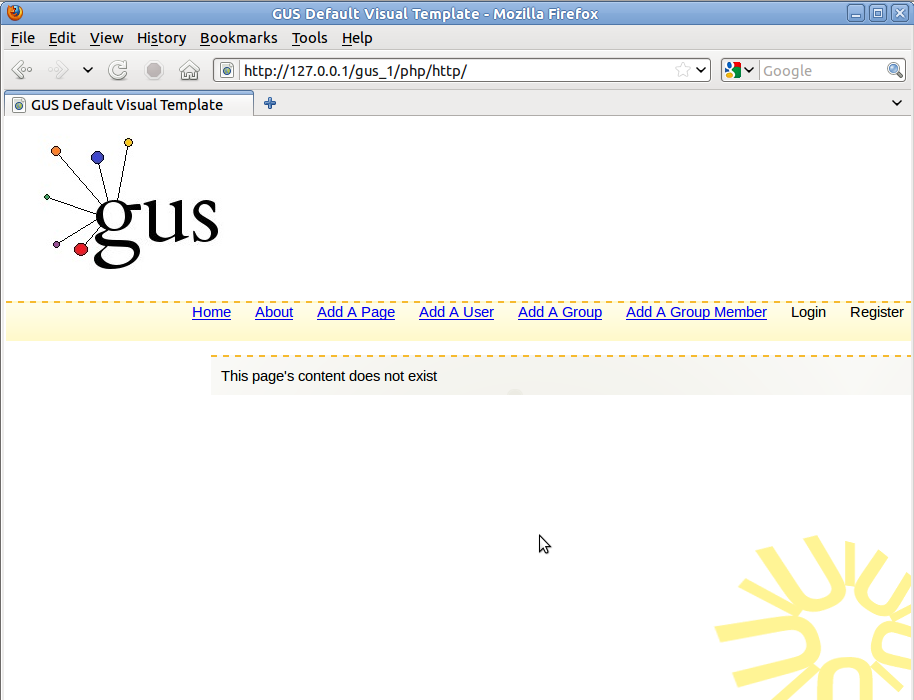
\includegraphics{'../http/png/index.png'}

Prepared for: \\
The Associated Students of the University of Idaho and Dr. Clinton Jeffery \\
Prepared by: \\
The PHP Gus Development Group \\
University of Idaho \\
Moscow, ID  83844-1010 \\
CS383 SSDD
\end{center}
\pagebreak
\tableofcontents
\liststyleWWviiiNumiii

\clearpage\setcounter{page}{1}\pagestyle{Convertiv}

\section{Introduction}
	\subsection{Identification}
The software under development is referred to as Groups in a
University Setting (GUS).  The customers providing specifications for the PHP
team are the student groups at the University of Idaho.  The  end users will be
of GUS will be the students and student groups at the University of Idaho.
This is a new product effort, so the version under development is version 0.004.
	\subsection{Document Purpose, Scope, and Intended Audience}
		\subsubsection{Document Purpose}
The purpose of this document is to describe the design of GUS.  This document
will serve as a guide for the PHP team as they move forward in development.
After the product is completed, this document will serve as a reference in
maintaining and updating the product.
		\subsubsection{Document Scope}
This document aims to contain the documentation needed to develop GUS.
It will include UML diagrams, use case descriptions and other important
details with regards to the design of the product.
		\subsubsection{Intended Audience for Document}
This document is intended to be read by the development team, the team's sponsor Dr.
Jeffery, and any personnel responisble for performing maintenance on or updating GUS.
While the system will be used by university personnel, this document is
intended to be read and understood by UICS software designers and coders.
This document will also be approved by Dr. Clinton Jeffery.

	\subsection{System Software Purpose, Scope, and Intended Users}
		\subsubsection{System and Software Purpose}
The purpose of the system under development is to provide a utility to groups
at the University of Idaho for administration and communication purposes.  GUS will
allow students to connect with groups that will meet their involement needs.
The system will be used by clubs, sports teams, and other university groups to
increase student involvement by connecting and recognizing the involvement of members.
		\subsubsection{System and Software Scope/or Context}
The finished product will run on University of Idaho servers and will be accessible
from any computer with a web browser and Internet access.  A user will be able to
log in and receive updates and communications from their groups anytime it is
convenient for the user.
		\subsubsection{Intended Users for the System and Software}
The intended users of the system are students and student groups at the
University of Idaho.

\newpage
	\subsection{Definitions, Acronyms, and Abbreviations}

\begin{flushleft}

\tablehead{\hline
\textbf{Term or Acronym}
&\textbf{Definition}
\\\hline}
\begin{supertabular}{|m{1.3587599in}|m{5.0011597in}|}
Acquirer & The person, team, or organization that pursues a system or software
product or service from a supplier. The acquirer may be a buyer, customer, owner,
purchaser, or user. ISO/IEC 42010:2007 (�3.1).\\\hline
AD & Architectural Description: A collection of products to document an
architecture ISO/IEC 42010:2007 (�3.4).\\\hline
Alpha test & Limited release(s) to selected, outside testers\\\hline
Architect & The person, team, or organization responsible for systems
architecture ISO/IEC 42010:2007 (�3.2).\\\hline
 Architectural Description &
 (AD) A
collection of products to document an architecture
ISO/IEC 42010:2007 (�3.4).\\\hline
 Architectural View &

{A
representation of a whole system from the perspective of a related set
of concerns ISO/IEC 42010:2007 (�3.9).}\\\hline
 Architecture &

{The
fundamental organization of a system embodied in its components, their
relationships to each other, and to the environment, and the principles
guiding its design and evolution ISO/IEC 42010:2007
(�3.5).}\\\hline
 Beta test &
 Limited release(s) to cooperating
customers wanting early access to developing systems\\\hline
 Design Entity &

{An
element (component) of a design that is structurally and functionally
distinct from other elements and that is separately named and
referenced IEEE STD 1016-1998 (�3.1).}\\\hline
 Design View &

{A
subset of design entity attribute information that is specifically
suited to the needs of a software project activity
IEEE STD 1016-1998 (�3.2).}\\\hline
 Final test &
 aka, Acceptance test, release of
full functionality to customer for approval\\\hline
 DFD &
 Data Flow Diagram\\\hline
 SDD &
 Software Design Document, aka SDS,
Software Design Specification\\\hline
 Software Design Description &

{A
representation of a software system created to facilitate analysis,
planning, implementation, and decision making, A blueprint or model of
a software system. The SDD is used as the primary medium for
communicating software }{design
information IEEE STD 1016-1998 (�3.4).}\\\hline
 SRS &
 Software Requirements
Specification\\\hline
 SSDD &
 System and Software Design
Document\\\hline
 SSRS &
 System and Software Requirements
Specification\\\hline
 System &

{A
collection of components organized to accomplish a specific function or
set of functions ISO/IEC 42010:2007
(�3.7).}\\\hline
 System and Software Architecture
and Design Description &
 An architectural and detailed
design description that includes a software system within the context
of its enclosing system and describes the enclosing system, the
enclosed software, and their relationship and interfaces.\\\hline
 System Stakeholder &

{An
individual, team, or organization (or classes thereof) with interests
in, or concerns, relative to, a system ISO/IEC
42010:2007 (�3.8).}\\\hline

\end{supertabular}

\end{flushleft}
\newpage
\subsection[DOCUMENT
REFERENCES]{\bfseries DOCUMENT
REFERENCES}

\liststyleWWviiiNumii
\begin{enumerate}
\item {{CSDS,}{\textit{System and Software Requirements Specification Template}}
{, Version 1.0, July 31, 2008, Center for Secure and Dependable Systems,
University of Idaho, Moscow, ID, 83844.}}
\item {{ISO/IEC/IEEE,}{\textit{IEEE Std 1471-2000 Systems and software
engineering -- Recommended practice for architectural description of software
intensive systems,}}{First edition 2007-07-15,  International Organization for
Standardization and International Electro-technical Commission, (ISO/IEC), Case
postale 56, CH-1211 Gen�ve 20, Switzerland, and The Institute of Electrical and
Electronics Engineers, Inc., (IEEE), 445 Hoes Lane, Piscataway, NJ 08854, USA.}}
\item {{IEEE, }{\textit{IEEE Std 1016-1998 Recommended Practice for Software
Design Descriptions}}{, 1998-09-23, The Institute of Electrical and Electronics
Engineers, Inc., (IEEE) 445 Hoes Lane, Piscataway, NJ 08854, USA.}}
\item {{ ISO/IEC/IEEE,}{\textit{IEEE Std. 15288-2008 Systems and Software
Engineering -- System life cycle processes,}}{ Second edition 2008-02-01,
International Organization for Standardization and International Electro-technical
Commission, (ISO/IEC), Case postale 56, CH-1211 Gen�ve 20, Switzerland, and The
Institute of Electrical and Electronics Engineers, Inc., (IEEE), 445 Hoes Lane,
Piscataway, NJ 08854, USA.}}
\item {{ISO/IEC/IEEE, IEEE Std. 12207-2008,}{\textit{Systems and software
engineering -- Software life cycle processes, }}{Second edition 2008-02-01,
International Organization for Standardization and International Electro-technical
Commission, (ISO/IEC), Case postale 56, CH-1211 Gen�ve 20, Switzerland, and The
Institute of Electrical and Electronics Engineers, Inc., (IEEE), 445 Hoes Lane,
Piscataway, NJ 08854, USA.}}
\end{enumerate}
	\subsection{Document Overview}
		\subsubsection{Section 2}
This section of the document describes the system and software constraints
imposed by the operational environment, system requirements and user
characteristics, and then identifies the system stakeholders and lists
and describes their concerns and mitigations to those concerns.
	\subsubsection{Section 3}
This section of the document describes the system and software architecture from several
viewpoints, including, but not limited to,the developer{\textquoteright}s view and the
user{\textquoteright}s view.
	\subsubsection{Section 4}
This section of the document provides detailed design descriptions for every component defined in the
architectural view(s).
	\subsubsection{Sections 5}
This section of the document provides traceability
information connecting the original specifications (referenced above)
to the architectural components and design entities identified in this
document.
	\subsubsection{Section 6}
Section 6 and beyond are appendices including original
information and communications used to create this document.

\subsection{Document Restrictions}
This document is for LIMITED RELEASE ONLY to University of Idaho CS personnel
working on the project and Dr. Jeffery.

\section{Constraints and Stakeholder Concerns}
	\subsection{Constraints}
		\subsubsection{Environmental Constraints}
GUS must be maintained in a secure office to prevent unauthorized
physical access to the server.  The office should be located
in an area that is unlikely to suffer from natural disasters, such as
flooding, earthquakes, etc.  The system should also be able to withstand
frequent power outages in case of wind storms.
		\subsubsection{System Requirement Constraints.}
Since users will access GUS through the Internet, GUS needs to be able to
maintain a constant connection to the Internet.  GUS will also need to
be able to interface with any data source it needs information from, such as
databases, web authentication servers, and users.  It will also need to keep
this information secure and confidential when appropriate.
		\subsubsection{User Characteristic Constraints.}
GUS will be easy for any user to understand after a brief explanation.
Even without an explanation, users will be able to determine the usage
and functionality of the system by looking through the options.
Basic computer skills and a simple conceptual explanantion
should be enough for everyday usage.
\begin{landscape}
	\subsection{Stakeholder Concerns}
\begin{flushleft}
\tablehead{\hline
\multicolumn{4}{|m{9in}|}{\centering
\bfseries Stakeholder x Concern x
Mitigation Table}\\\hline
\multicolumn{1}{|m{1.3in}|}{\centering
{\bfseries Stakeholder}\par

\centering \bfseries Concern} &
\centering \bfseries List of
Stakeholders &
\centering \bfseries Stated Concern
&
\centering\arraybslash \bfseries
Mitigation Mechanism or Design Criteria Reference Number
\\\hline}
\begin{supertabular}{|m{1.2in}|m{.9in}|m{2.6in}|m{3.6in}|}

\multicolumn{1}{|m{1.2in}|}{Appropriateness of the system and}
 & Acquirer
 & Will this project develop the software engineering skills required to work in the industry?
 & Limit the size of the teams, require developers to use server-side scripting and extensive development documentation
 \\\hhline{~---}
 software in fulfilling its mission
 & User
 & Will this system be user friendly enough that a computer illiterate person can use it?
 & Provide visual and textual cues to make it easy for non-technical users to understand
\\\hline
\multicolumn{1}{|m{1.2in}|}{
Feasibility of constructing, testing, }
 & Developer
 & Will this project be interesting and completable within one semester?
 & Encourage members to work on the parts of the project they are interested in, and share the workload.
\\\hhline{~---}
verifying and deploying the
system and software.
 & Tester
 & Will the testing utilities be user-friendly enough to learn without spending too much time?
 & Collectively identify appropriate testing utilities for each platform the testers will be using, and identify helpful tutorials
\\\hline
Risks of constructing, deploying, and
 & Acquirer
 & Will this system make the University of Idaho legally liable if the system is hacked?
 & Educate users of the risks of posting private information on the Internet, and limit the information GUS tracks
\\\hhline{~---}
\multicolumn{1}{|m{1.2in}|}{using the system and software object of this SSDD.}
 & User
 & Will my information be kept private from stalkers, telemarketers, and other creeps?
 & Use security measures, such as keeping GUS physically secure, encrypting information,
 and using modular \textbf{mutually suspicious programming}
\\\hline
Concerns with respect to the maintainability and
 & Acquirer
 & Will there be a maintainer?
 & Include Dr. Jefferey in every step of the design process, and try to fill an important niche for the University of Idaho
\\\hhline{~---}
\multicolumn{1}{|m{1.2in}|}{evolvability of the system and software.}
 & Maintainer
 & Will GUS be easy to port to another system that would maintain it?
 & Keep all aspects of GUS extremely simple and practice good coding to enable portability
\\\hline
\end{supertabular}
\end{flushleft}
\end{landscape}
\pagebreak
\section{System and Software Architecture}

\subsection{Developer{\textquoteright}s Architectural View}
The basic architecture of GUS is a database driven, client-server web application.
The components of GUS are: graphical user interfaces (websites), web-interfaces to a database, and a database.
The graphical user interfaces are the only part the user directly sees and manipulates.  They allow users to input
and view information in the database and they communicate with the web-interfaces to access the database
and present the data in a human-readable form.  The web interfaces ensure that the input from
the users is valid and safe to put in the database, and they also ensure that data pulled from
the database is sent only to the appropriate users.

\subsection{User{\textquoteright}s Architectural View}
GUS is a website with different levels of privelege for users, officers, and administrators.
When logged into GUS, a user will have member-level access to groups that they are a member of,
officer-level access for groups they are an officer in, and administrative privileges for
groups they own.

\subsubsection{User{\textquoteright}s View Identification}
From the user{\textquoteright}s point of view, GUS is a tool that enables users to connect
with one another through groups.  As such, communication between users is a very important component
and is fulfilled by several different modules including e-mail and forums.  One of the major
distinctions between users in a group is their level of privilege, and there are specific modules
for each of the three levels of privelege.

%I think the figures and use cases need to be moved/reworked/reogranized
%Replace User's View Representation and Description with module name?
%Rather than 3.2.2.1.1 etc. should be 3.2.2.1 or something.
%Better yet, use real paragraphs rather than subsections?

\begin{wrapfigure}[12]{r}{2in}
  \begin{center}
    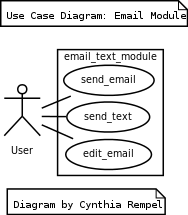
\includegraphics{'../pdf_png/email_use_cases.png'}
  \end{center}
  \caption{Replace with screenshot of email mock-up}
\end{wrapfigure}


\subsubsection{User{\textquoteright}s View Representation and Description}

\\{\bf Text and E-mail Module}

\\User-view class diagram which this entry is based on was designed by Brett Hitchcock,
this entry was written by Cynthia Rempel.

\\The purpose of the e-mail module is to enable users to send e-mails to groups and other users.
Two advantages of using GUS to communcate are: texting and predefined social networks.
The texting feature enables users or groups to communicate about events at the last minute via SMS
text messages.  Instead of each user manually updating their e-mail lists when people leave the group,
GUS tracks the members for each group. For example: the president of the Business Professionals of America
might want to invite the Information Systems club to a meeting about their information systems competitive events.
Another example: the president of the Tech club cancels a meeting at the last minute because
the advisor is ill, and he texts all of the Tech club members.
A user can access their e-mail and text features through their e-mail page, and
they can only text people (or groups) that have  permission to e-mail or text.


\pagebreak

\paragraph{Forums Module}
\begin{wrapfigure}[17]{l}{2in}
  \begin{center}
    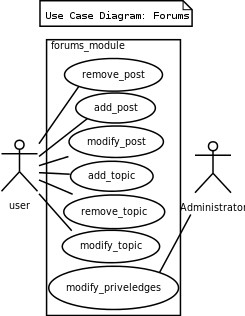
\includegraphics{'../pdf_png/forums_use_cases.png'}
  \end{center}
  \caption{replace with screen-shots of forums mock-ups}
\end{wrapfigure}
\subparagraph{}--- diagram which this entry is based on was designed by ---, this entry was written by Cynthia Rempel.
\subparagraph{} The forums module is designed to enable groups to collaborate on group decisions and consolidate member input.
For example: the president of the tech-club may start a forum on brainstorming and developing informal business plans to raise money.
From there, the vice president might post a topic of using the club to start computer repair shop, the secretary may line out possible services,
the treasurer may suggest a fee schedule, and members may volunteer what services, and how much time they could commit to the idea.

\subparagraph{} To post on the forums page a user would have to be granted permissions by the groups administrator,
and the user would have to be on the groups forum page.  Types of permissions a user would expect to see are: add post, modify own post,
modify other members posts, remove own post, and remove other members posts;
{there would be a similar (but possibly more restrictive) set of permissions for topics.}\\
\subparagraph{} {For the administrator to modify privaledges, she should be on the forums page of the group, ideally,
there should be some minimal guidance on the security aspects of giving users permissions right on the forums page,
perhaps a \textbf{permissions wizard} }\\

\begin{wrapfigure}[17]{r}{2in}
  \begin{center}
    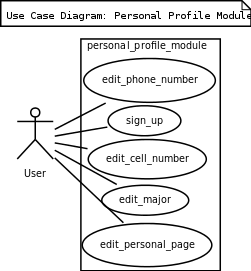
\includegraphics{'../pdf_png/profile_use_cases.png'}
  \end{center}
  \caption{replace with screen-shot of profile mock-up}
\end{wrapfigure}
\paragraph{Profile Module}

\subparagraph{} The user-view class diagram which this entry is based on was designed by Brett Hitchcock,
this entry was written by Cynthia Rempel.\\

\subparagraph{} The purpose of a profile is to enable the user or group to present a picture of who she or they are,
so other users or groups can make an informed decision of whether to associate with her or them.

For example: the Business Professionals of America (BPA) club might appeal to the Virtual Technology and Design (VTD) majors,
because BPA displays their video animation competive event for which they want to recuit judges at the local high-school level
and participants at the college-level. Also, the Lutheran Campus Ministry might want to attract music majors,
because of their proximity to the Music building. Another example of a profile feature might be an incoming freshmen might be
really interested in video games, and the video game club is looking for members.\\

\subparagraph{}
Users may want the amount of information shared limited to only a subset of groups they are members of.  For example: Joan2833 may want to
share her schedule with members of the National Youth Accreditation Association (NYACC), but not with ASUI.\\
\subparagraph{} The personal profile is also a way for users to keep their information up-to-date.  For example: if the head coach needs
to contact the Tech club president for last minute changes for the awards to be engraved (the underdog pulled through at the last minute)
and so his name is to be engraved now.  Another example would be, every fall the ASUI emails all the student groups with the times for
mandatory officer orientation, and up-to-date emails facilitate this process.\\
\begin{wrapfigure}[24]{r}{4in}
	\begin{center}
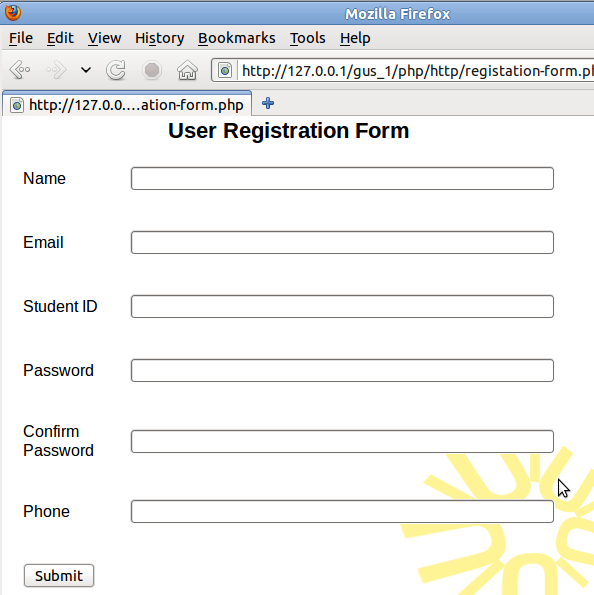
\includegraphics{'../http/png/registration-form.png'}
	\end{center}
	\caption{registration form by Abhay Patil}
\end{wrapfigure}
\subparagraph{} Use case: register for gus\\
\textbf{Actor:} prospective user \\
\textbf{Goal:} user will be registered for GUS\\
\textbf{Preconditions:} user is at GUS registration page\\
\textbf{Related Use Cases:} edit personal information\\
\textbf{Steps:}\\
1. User enters their name\\
2. User enters their email\\
3. User enters their user name\\
4. User enters their password\\
5. User enters their password again\\
6. User enters their phone number\\
7. User clicks submit\\
\textbf{Alternatives:} user navigates away from page, officer or administrator may desire to add a user who is less technically literate\\
\textbf{Post Conditions:} The user's name, email, user name, password,
and phone number are validated, and then sent to GUS to be put in the database\\
\begin{wrapfigure}[15]{l}{200px}
  \begin{center}
    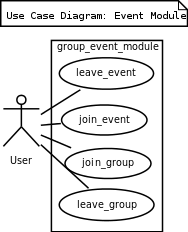
\includegraphics{'../pdf_png/event_use_cases.png'}
  \end{center}
  \caption{Replace with mock-up of a page inviting the user to join a group and/or an event}
\end{wrapfigure}
\paragraph{Event Group Module}
\subparagraph{} The user-view class diagram which this entry is based on was designed by Brett Hitchcock,
this entry was written by Cynthia Rempel. \\

\subparagraph{} The purpose of the event group module is to enable users to join groups and events.
Users can use GUS to look for groups that interest them, or they might want to join events that interest them.
For example: a softmore interested in becoming a Methodist minister may decide joining Religion and Ethics may look really good on
an application to go to seminary.
A marketing major may want to sign up to judge at a DECA event that Business Professionals of America is hosting to
encourage high-schoolers to learn business skills.
\pagebreak
\begin{wrapfigure}[23]{r}{4in}
  \begin{center}
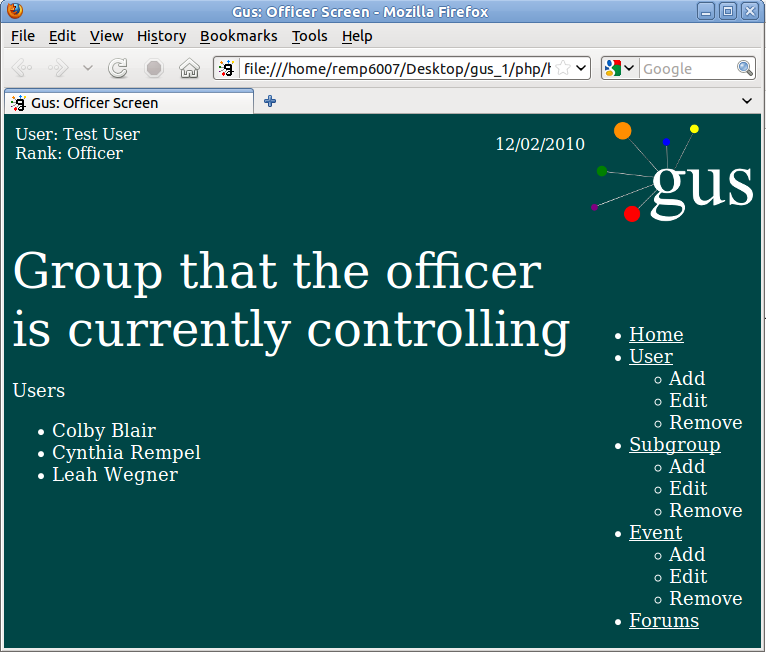
\includegraphics{'../http/png/officer_control.png'}
  \end{center}
  \caption{Officer Panel Mockup by Leah Wegner}
\end{wrapfigure}
\paragraph{Officer Module}
\subparagraph{} The purpose of the officer module is to enable officers to manage the group events, membership, and website.
For example, the president of the UI Tech club could post a plaque engraving event for 2:30 PM, and after 10 people signed up, there could be a snowstorm
(2 ft in one hour!) at 12:30 he cancels the event, so he decides to send a group text (which includes not only UI Tech club members
likely to attend but didn't sign up,
but everyone who RSVPed to include John (who's just taking the class and is not in club), followed up by an email, and finally the president
prints out a roster of the likely attenders who only have a land-line with no internet to call manually.
John later decides to join the Tech club, and the treasurer uses GUS to add him to the Tech club.\\
\subparagraph{} An officer may want to change the contents of a group's web page.  For example: this year Idaho's Business
Professionals of America State Leadership Conference is holding a C++ event, and BPA may want to add that back to their group page.\\
\begin{wrapfigure}[19]{l}{3in}
  \begin{center}
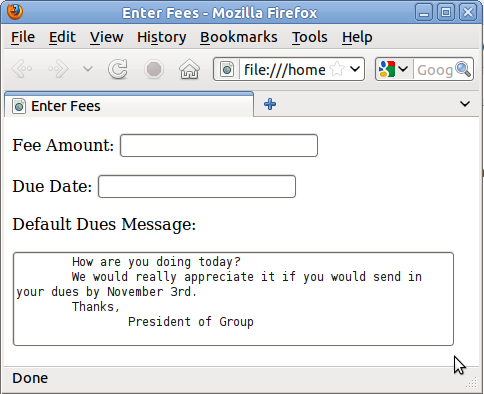
\includegraphics{'../http/user_mockups/enter_fees_mockup.png'}
  \end{center}
  \caption{Enter Fees Mockup by Cindy}
\end{wrapfigure}
\subparagraph{}Use case: enter fee information\\
\textbf{Actor:} officer \\
\textbf{Goal:} Store group dues in GUS databse \\
\textbf{Precondtitions:} Officer is logged on and at the group's officer page\\
\textbf{Related use cases:} Remind users to pay dues, enter membership criteria \\
\textbf{Steps:}\\
1. Click 'enter fee information'\\
2. Type in fee amount\\
3. Select due date from a calendar\\
4. Click 'save' \\
\textbf{Alternatives:} \\
\textbf{Postconditions:} the dues information is saved in the database \\
This use-case can be expanded by using the same screen for an officer to specify
all the membership criteria: waivers, dues, service project, class standing, GPA, major, etc.\\
\pagebreak
\begin{wrapfigure}[24]{l}{3in}
  \begin{center}
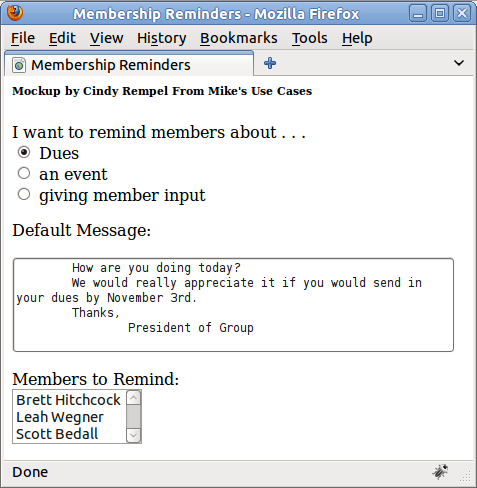
\includegraphics{'../http/user_mockups/notify_concerning_fees_mockup.png'}
  \end{center}
  \caption{Membership Reminders Mockup by Cindy}
\end{wrapfigure}

\subparagraph{Use case: notify members concerning dues/fees} from Mike's use cases.

\textbf{Actor:} group leader \\
\textbf{Goal:} notify members of outstanding expenses \\
\textbf{Precondtitions:} expense information is already entered into GUS\\
\textbf{Related use cases:} enter fee information, send message, notify members to fill out waivers\\
\textbf{Steps:}\\
1. Click 'money'\\
2. Click 'send notifications'\\
3. Write a reminder message or use the default dues reminder message \\
4. Choose the users who need to be reminded (perhaps GUS could be used to store who has paid dues and who hasn't) \\
\textbf{Alternatives:} the officer cancells out of the usecase by clicking elsewhere, perhaps this use-case could be expanded to allow
the officer to remind members about multiple membership criteria they need to meet, but personalized so members are only reminded of what
they are deficient in.\\
\textbf{Postconditions:} a notification is emailed to each applicable member \\

%\begin{wrapfigure}{r}{200px}
%  \begin{center}
%    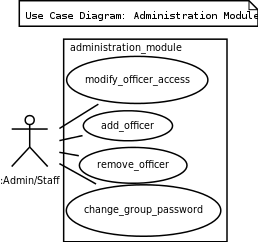
\includegraphics{'../pdf_png/admin_use_cases.png'}
%  \end{center}
%\end{wrapfigure}
%\paragraph{Administrative Module}
%\subparagraph{} The purpose of the administrative module

\subsubsection{Developer{\textquoteright}s View Representation and
Description}
\paragraph{} GUS is made of three basic systems, the user interface (forms class),
the interface between the user interface and the database (GUS class),
and the calls to the database (MySql class).
The forms class collects data from users, then hands the data to GUS, which in turn,
transmits the data to the database. When a user makes a request for data, GUS queries the database,
prepares the information to be displayed, and the forms class displays the information.
The forms class can be extended to have additional text fields for user input.
The GUS class establishes a connection to the database for the transfer of data,
and uses that data to set up page content for the user. The MySql class connects and disconnects from GUS,
implements the database design, queries the database, and enables GUS to make changes to the database.
\begin{figure}[ht]
    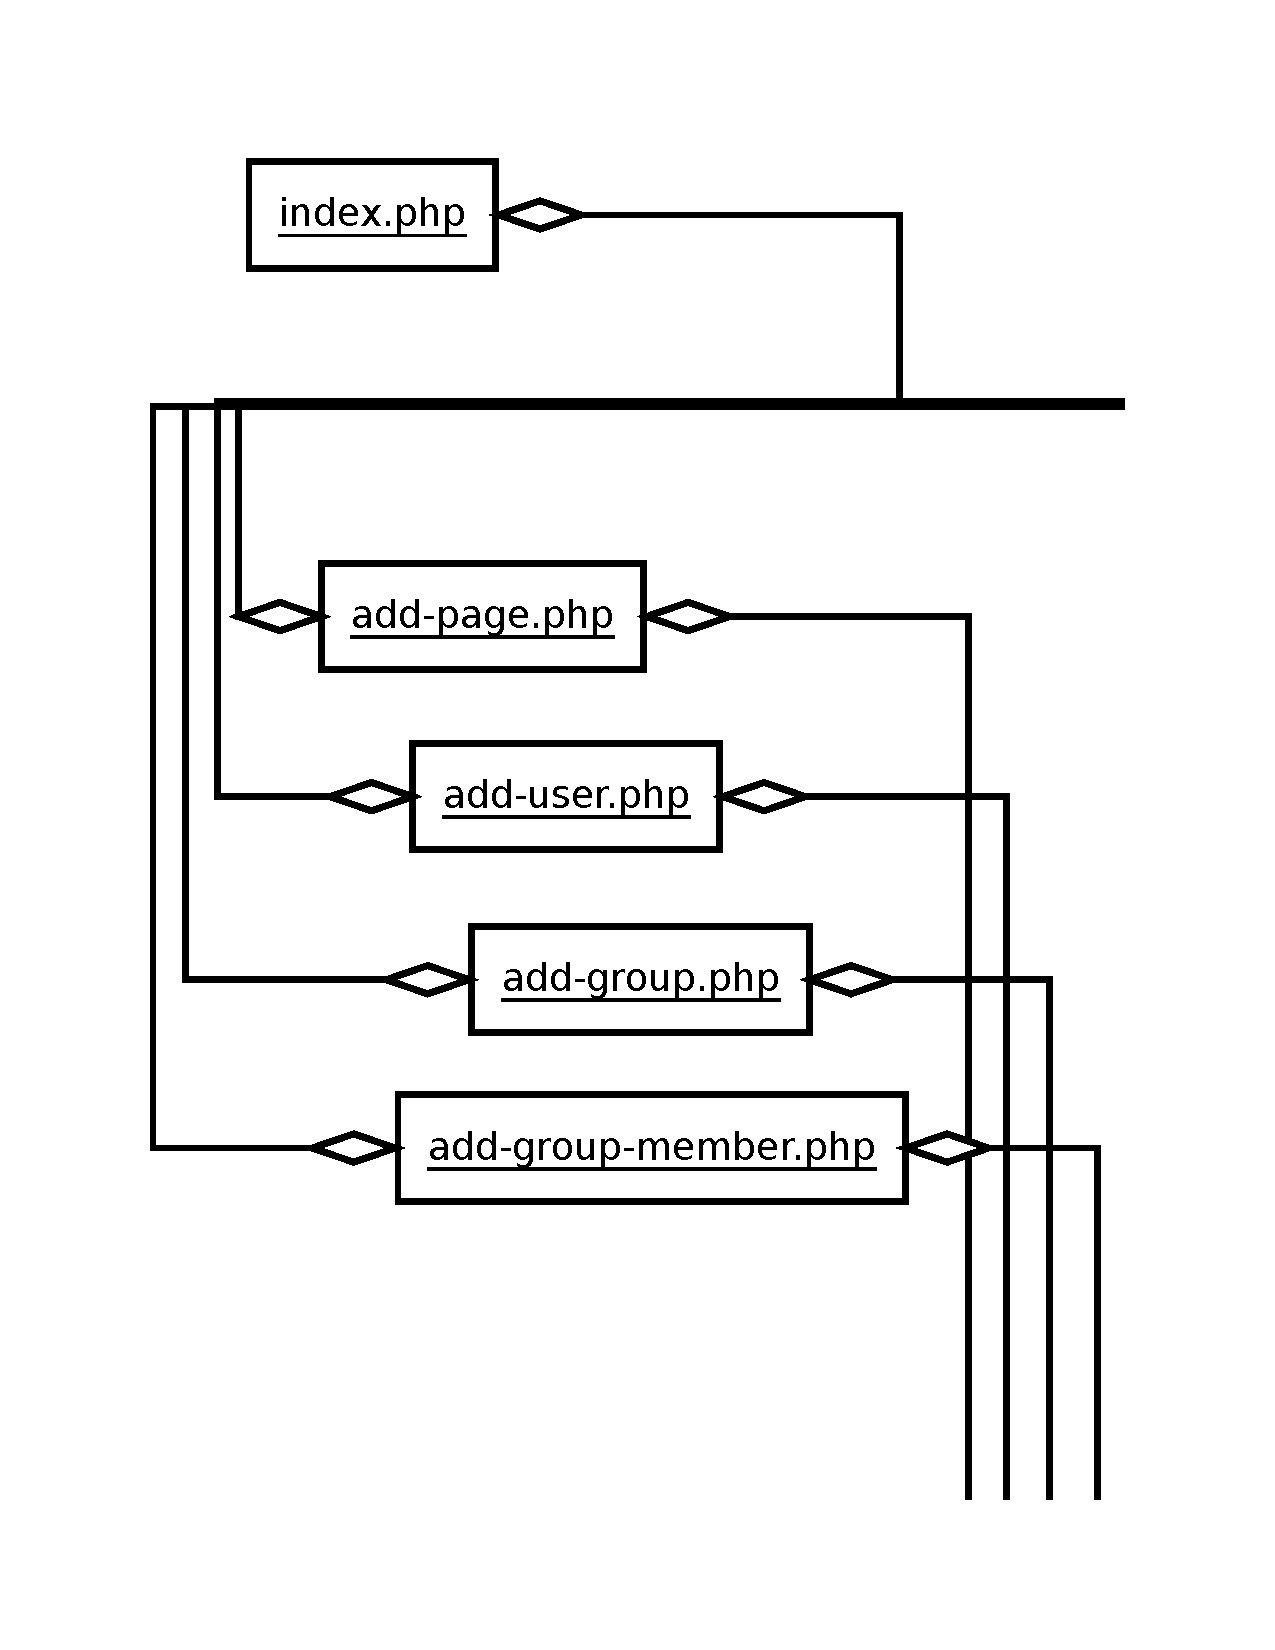
\includegraphics{'../doc/proto_framework_associations.png'}
	\caption{Prototype Framwork Associations by Colby Blair}
\end{figure}


\subsubsection{Developer{\textquoteright}s Architectural Rationale}


\subsection[\ [ insert name of viewpoint {]} ARCHITECTURAL
VIEW]{{ }{[ insert
name of viewpoint ] ARCHITECTURAL VIEW}}
{\itshape
This subsection contains the descriptions of a system and all of its
major components, using the methods, techniques, and languages from
other than the developer{\textquoteright}s or user{\textquoteright}s
viewpoint.  Each viewpoint description includes the viewpoint
identification, description, and diagrammatic representation. }

{\itshape
Repeat this subsection for each viewpoint identified.}

\subsubsection{[ insert name of viewpoint ]{\textquoteright}s View
Identification}
{\itshape
Identify the view, state the purpose of the view, and identify major
components or processes of the architecture.}

{
[Insert text here.]}

\subsubsection{[ insert name of viewpoint ]{\textquoteright}s View
Representation and Description }

{
[Insert diagram and descriptions here.]}

\subsection[CONSISTENCY OF ARCHITECTURAL
VIEWS]{\bfseries CONSISTENCY OF
ARCHITECTURAL VIEWS}
{\itshape
For compliance with ISO/IEC 42010:2007 (�5.5) an Architectural
Description (AD) shall include a list of all known inconsistencies
between the architectural views and an analysis of consistency across
all the architectural views.}

\subsubsection{Detail of Inconsistencies between Architectural Views}
{
[Insert text and graphics here.]}

\subsubsection{Consistency Analysis and Inconsistency Mitigations}
{\itshape
For each inconsistency identified above, provide solutions or
mitigations that resolve potential conflicts between the stakeholder
viewpoints.}

{
[Insert text or table here.]}

\section{Software Detailed Design}

\subsection{Developers Viewpoint Detailed Software Design}




\begin{landscape}
	\subsection{Component Dictionary}
\begin{flushleft}
\tablehead{\hline
\multicolumn{5}{|m{9in}|}{\centering
\bfseries Component Dictionary}\\\hline

\centering \bfseries Name &
\centering \bfseries Type/Range &
\centering \bfseries Purpose/Function
&
\centering\arraybslash \bfseries
Dependencies
& Subordinates
\\\hline}
\begin{supertabular}{|m{1.75in}|m{1in}|m{1.75in}|m{3.25in}|m{1in}|}
Form
 & web-page
 & graphical user interface
 & requires GUS to transmit data back and forth to database
 & NA
\\\hline
GUS
 & web-server
 & interface between users and database management system
 & requires users to enter data and requires the MySql database to manage data
 & NA
\\\hline
MySql
 & database management system
 & maintain information, such as, user details, and student group organizations
 & requires GUS to transmit data back and forth from users
 & NA
\\\hline

\end{supertabular}
\end{flushleft}
\end{landscape}

\subsection{Component Detailed Design}
\subsection{Developer{\textquoteright}s View Identification}{}

	\subsubsection{Detailed Design for Component: Forms}
	The forms.php was written by Colby Blair, the section was reverse-engineered by Cynthia Rempel
	\paragraph{Introduction to Forms}
Users can use forms to tell GUS what is needs to know; their personal information,
such as names, majors, phone numbers, etc.; what groups they want to join;
allow users to post to forums; and any other data a user might want to input into GUS.
Forms also display data organized by the MySql class in a way that is meaningful for example:
a forum organized by topic and then chronologically, or an organization chart for a group.
\paragraph{Input for Forms}
\begin{enumerate}
\item textual user input
\item content from the GUS class
\end{enumerate}

\paragraph{Output for Forms}
\begin{enumerate}
\item content for GUS class
\item information displayed on a web page
\end{enumerate}

\paragraph{Forms Process to Convert Input to Output}
Forms collects user input by using \textbf{text-fields}, into an attribute called \textbf{content},
which is then collected by GUS.  Forms also takes \textbf{content} from GUS and displays it to users through \textbf{text-field}s.\\

\paragraph{Design constraints and performance requirements for Forms}
Forms must encrypt passwords, and only transmit sensitive data through secure protocols.
Forms must collect the minimum amount of data about a user to meet the mission of
student group organization and recruitment to minimize the desirability of GUS as a target for maliciousness.
\begin{figure}[ht]
    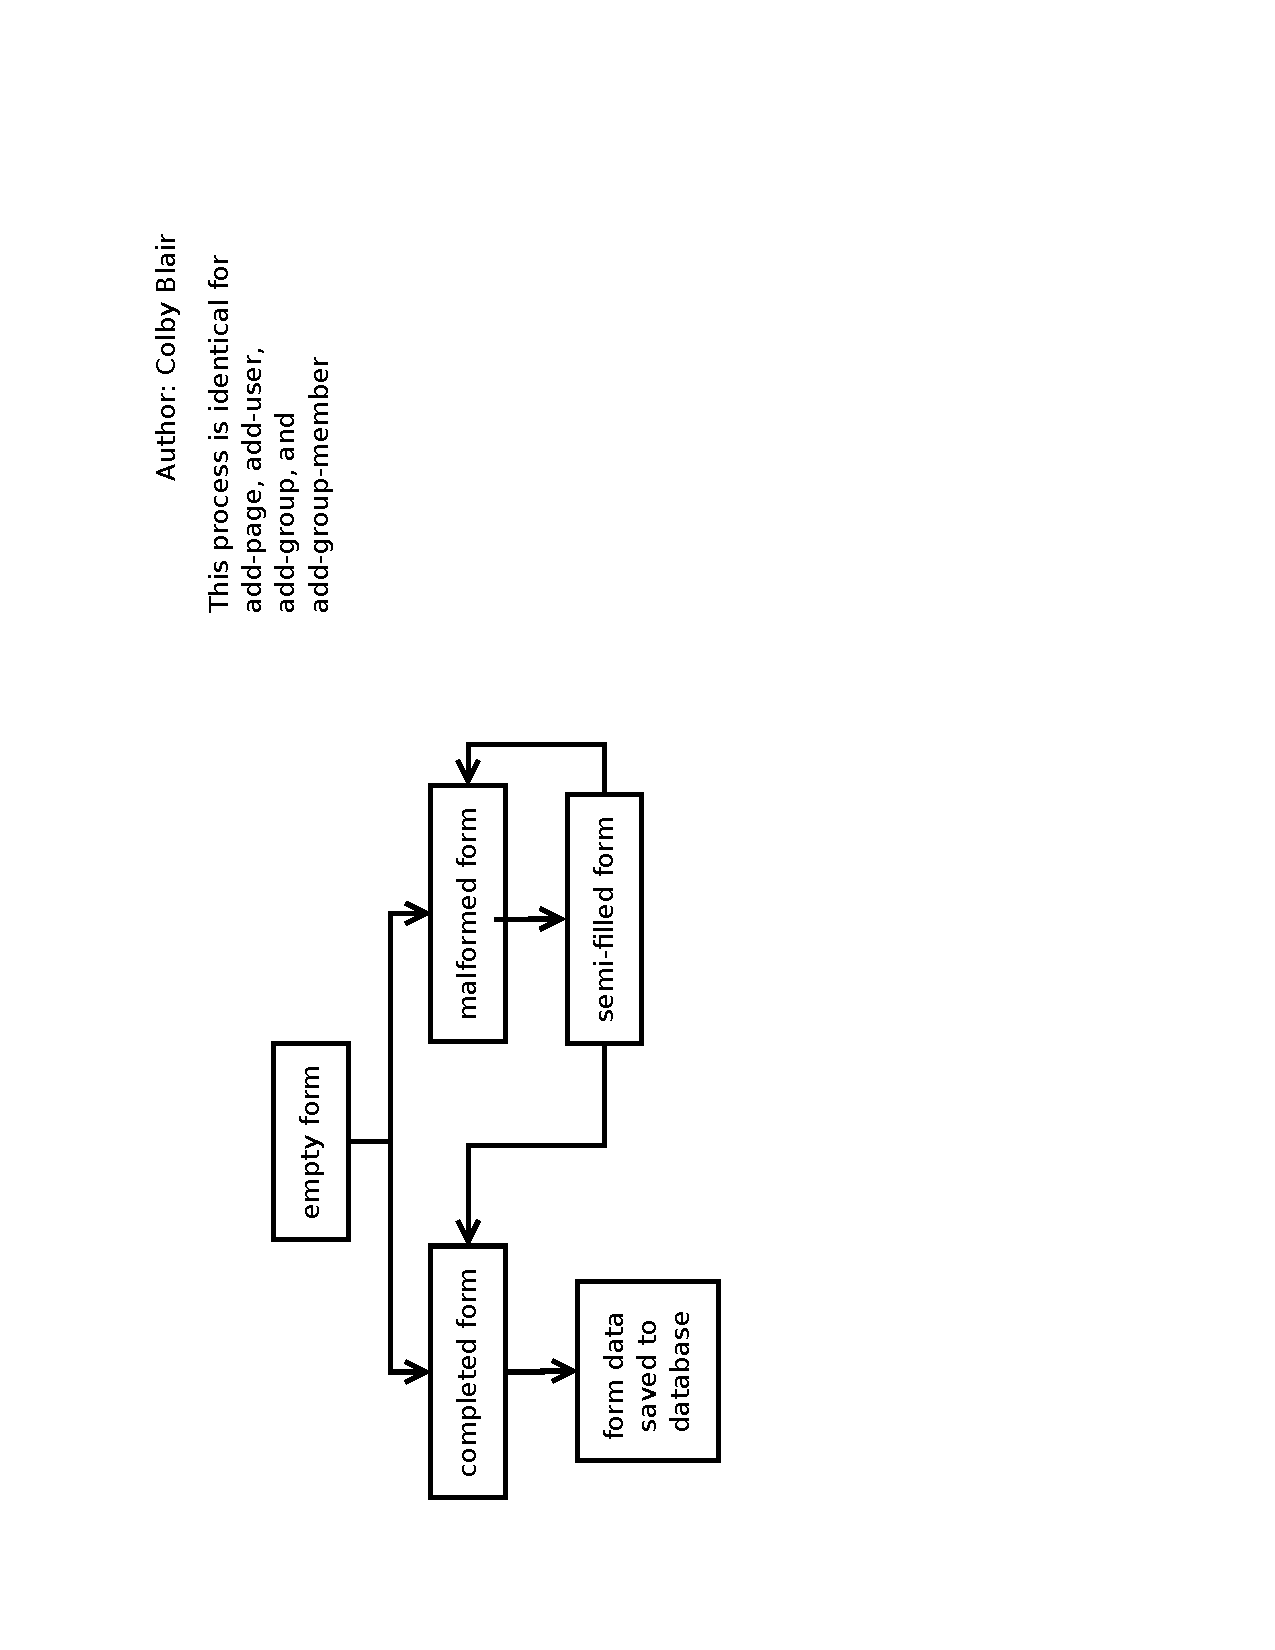
\includegraphics{'../doc/form-data-submission-statechart.png'}
	\caption{Form Submission Statechart by Colby Blair, transition descriptions by Cynthia Rempel}
\end{figure}
\subsubsection{Detailed Design for Component: GUS}
	The gus.php was written by Colby Blair, the section was reverse-engineered by Cynthia Rempel
\paragraph{Introduction to GUS}
GUS uses a \textbf{visual template} and a \textbf{database connection} to initiate a database connection, and set-up page content.
The visual template attribute is used to translate information obtained through the database connection into a user friendly format.

\paragraph{Input for GUS}
\begin{enumerate}
\item content from a form
\item content from the database connection
\end{enumerate}

\paragraph{Output for GUS}
\begin{enumerate}
\item a visual template for a web-page (if it's going to the user)
\item database entries (if it's going to the database connection)
\end{enumerate}

\paragraph{GUS Process to Convert Input to Output}
\begin{enumerate}
\item Initialize Database Connection (\textbf{init-db}) this private function establishes a connection with the
database by creating a new MySql object that has the correct data base host, admin, and uses the correct password.
\item Initialize Data (\textbf{init-data}): this private function queries the database through the database connection
to set-up a visual template.  It returns the first result, or if there is no result, it returns the original visual template.
\item Page Content (\textbf{page-content}): this public function gets a visual template (or makes one),
and queries the database to find a web-page.  If the page doesn't exist it returns an error message.
\end{enumerate}

\paragraph{Design constraints and performance requirements of GUS}
GUS must be able to handle incorrect user input, and deal with corrupt data from the database.

\subsubsection{Detailed Design for Component: MySql}
	The my.php was written by Colby Blair, the section was reverse-engineered by Cynthia Rempel
\paragraph{Introduction to MySql}
The MySql class uses a database connection (\textbf{db}) to: manage and query a database, and connect to GUS.

\paragraph{Input for MySql}
{
[ insert your text here ]}

\paragraph{Output for MySql}
{
[ insert your text here ]}

\paragraph{Component/Entity Process to Convert Input to Output}
\begin{enumerate}
\item Connect: this private function uses a \textbf{hostname},
a user-name (\textbf{un}), and a password (\textbf{pw}),
and returns a connection to GUS.
\item Disconnect: this private function closes the connection to GUS
\item Names and Values: this private function fills a \textbf{table}
with \textbf{data} and assigning that data \textbf{names} and
\textbf{values}
\item Where: this private function queries \textbf{data} in certain
fields (\textbf{use-fields}) in a \textbf{table} and returns a string
(\textbf{where}) with all the desired values.
\item Set: this private function cycles through all the \textbf{data}
in a \textbf{table} and returns a \textbf{set} of keys and values.
\item Exists: this private function takes the \textbf(names) and
\textbf(values) of the \textbf{table} and \textbf{data} and looks to see if the data exists
\item Error: this is an optional public error message function
\item Save: this public function goes through a table and updates the
\textbf{data}, \textbf{row} by row updating only the fields indicated.  The rows
that don't already exist in the table are inserted.
\item Select: this public function queries a \textbf{table} to get an
array of results \textbf{who} have the indicated attribute.
\item Select Condition (\textbf{select-cond}): this public function
cycles through all the rows in a table and returns all results
\textbf{who} meet the \textbf{cond}ition in the \textbf{table}.
\end{enumerate}

\paragraph{Design constraints and performance requirements of MySql}
The query language must be limited to the SQL dialect the database uses,
and the other side of the interface must be compatible with GUS.

\subsubsection{Detailed Design for the Installation Component:}
\paragraph{Introduction to Installation Component:}
The installation component sets up the database, and creates the tables: page, guser (gus user), ggroup (gus group)
ggroup-member (gus group member).
\paragraph{Input for the Installation Comnponent}
Although there are no explicit inputs it uses the following global parameters: the mode, the host's IP,
the admin's information, password, the database's name.  The choices for the mode are: MySql, LDAP, and file-driven.

\paragraph{Output for this Component/Entity}
Currently, the output for the installation module is a MySql database composed of tables.

\paragraph{Installation Process to Convert Input to Output}
The installation process connects to the host and uses a switch to identify the type of database, then the installation uses a CREATE DATABASE query,
and finally a series of CREATE TABLE queries.

\paragraph{Design constraints and performance requirements of the installation component}
The component must successfully connect to the host IP securely, without destroying any data, or compromising personal information.

\subsubsection{Detailed Design for Component: Add Group}
\paragraph{Introduction to Add Group}
Add group is designed to use a form to add a group to the GUS database.

\paragraph{Input for Add Group}
Add group takes the name and description of a group as input.

\paragraph{Output for Add Group}
A new entry in the ggroup (gus group) table.

\paragraph{The Add Group Process to Convert Input to Output}
Takes the name and description of the group and calls on the GUS interface to add the entry to the group table.

\paragraph{Design constraints and performance requirements of Add Group}
The only people that have authorization to add university groups are: ASUI, the Graduate and Professional Student Association,
and (possibly) the University of Idaho Student Bar Association.  Although it probably would be advisable to include the existing graduate,
professional, and legal student groups in the original installation and limit adding groups to just ASUI,
because there are very few new graduate and legal groups being added, and ASUI can assist the student bar and GPSA with adding those groups
(if they ever need to).
\subsubsection{Detailed Design for Component: Add Group Member}
\paragraph{Purpose of this Component}
Adds a member to the group membership table.

\paragraph{Input for this Component}
The input is the group ID and the user ID.

\paragraph{Output for this Component}
After this script is called an entry is made the group membership table.

\paragraph{Component/Entity Process to Convert Input to Output}
Hands the group ID and the user ID to the GUS interface to be processed and added to the group membership table.

\paragraph{Design constraints and performance requirements of this Component}
There should be a uniqueness constraint on user-ID and group-ID.  For example: although john2833 can be in both Business Professionals
of America (BPA) and the UI Tech Club, once he's in BPA, he should not get a second membership entry for BPA
if the BPA secretary accidently tries to add him when he is already in BPA.


\subsubsection{Detailed Design for the Main Component}
\paragraph{} The purpose of the main component is to identify the appropriate global parameters when installing GUS.
The parameters are the database mode (DBMODE), the database host (DBHOST), the database administrator (DBADMIN),
the default database user name (DBUN), the database password (DBPW), the database name (DBNAME), and the default
template directory (TMPLDIR).

\subsubsection{Detailed Design for Component: Uninstall}
\paragraph{Purpose of this Component:}
The purpose of this component is to uninstall GUS from a computer.

\paragraph{Output for Uninstall}
Uninstall removes the database.

\paragraph{Component Process to Convert Input to Output}
Connects to the database, and performs a DROP DATABASE command in MySql.

\paragraph{Design constraints and performance requirements of this Component}
Access to this feature should be very limited -- one command can remove an entire social network.\\

\begin{wrapfigure}{r}{375px}
  \begin{center}
    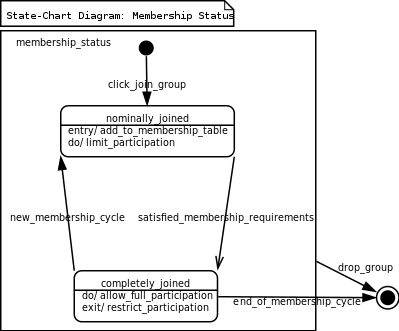
\includegraphics{'../pdf_png/membership_statechart.png'}
  \end{center}
\end{wrapfigure}
\subsubsection{Detailed Design for Entity: Membership Status}
\paragraph{Purpose of this Entity}
The purpose of membership status is to enable groups to give benefits to members who have earned them.  For example:
Business Professionals of America may require members to pay \$30 dues, sign a waiver, and assist with a fundraising event
\textbf{before} paying for the student to go to the State Leadership Conference.
\paragraph{Input for this Entity}
\begin{itemize}
\item a request from the member, officer, or administrator to change the status of the member
\item a triggering action, such as, paying dues, signing a waiver, or attending a mandatory meeting
\item the end of a membership cycle: such as, the end of the school-year, graduation, change in the groups staff
\end{itemize}
\paragraph{Output for this Entity}
If the conditions are met, a change in the membership table to reflect the change in the status.
\paragraph{Process to Convert Input to Output}
\subparagraph{} If a user makes a request, GUS checks to see if the user is authorized to make the requested change, if not, the user's
request is forwarded to the approving authority, if the group so desires.  If the user is authorized to make the change,
then the change is made in the table through a php call to the database.
\subparagraph{} If an authorized user checks off that a membership condition has been met, that information is stored in GUS.
GUS then checks to see if all membership criteria for the group has been met, if so, GUS updates the members status.
\paragraph{Design constraints and performance requirements}
Membership requirements would have to be unique to each group -- Lutheran Campus
\subsubsection{Detailed Design for Entity: Membership Status}
\paragraph[\ Introduction/Purpose of this Component/Entity]{
Introduction/Purpose of this Component/Entity}
{
[ insert your text here ]}

\paragraph{Input for this Component/Entity}
{
[ insert your text here ]}

\paragraph{Output for this Component/Entity}
{
[ insert your text here ]}

\paragraph{Component/Entity Process to Convert Input to Output}
{
[ insert your text here ]}

\paragraph{Design constraints and performance requirements of this
Component/Entity}
{
[ insert your text here ]}
\subsection{DATA DICTIONARY}
{\itshape
This subsection shall list and describe all the data and data structures
defined and/or used by the components and entities specified above.
For each data item or structure indicate where it is defined,
referenced, and modified.}

\begin{landscape}
	\subsection{Function Dictionary}
\begin{flushleft}
\tablehead{\hline
\multicolumn{5}{|m{9in}|}{\centering
\bfseries Function Dictionary}\\\hline
 Name
 & Type/Range
 & Defined By
 & Referenced By . . .
 & References
\\\hline}
\begin{supertabular}{|m{1.75in}|m{1in}|m{1.75in}|m{3.25in}|m{1in}|}
add-text-field
 &
 & 4.3.1.4
 &
 & name
 \\\hline
error
 & message
 &
 &
 &
\\\hline
init-db
 & GUS
 & 4.3.2.4
 &
 & ds, mysql
\\\hline
init-data
 & GUS
 & 4.3.2.4
 &
 & vt, mysql.select-cond
\\\hline
page-content
 & GUS
 & 4.3.2.4
 &
 & vt, ds.select-cond
\\\hline
construct
 & MySql
 &
 &
 & connect,
\\\hline

\end{supertabular}
\end{flushleft}
\end{landscape}

\section[REQUIREMENTS
TRACEABILITY]{\bfseries
REQUIREMENTS TRACEABILITY}
{
{\textit{This section shall contain
traceability information from each system requirement in this
specification to the system (or subsystem, if applicable) requirements
it addresses.  A tabular form is preferred, but not mandatory.
}}{\textit{A detailed mapping between
requirements and constraints in the SSRS and architectural components
and detailed entities in this SSDD is required. For compliance with
ISO/IEC 15288:2008
}}{\textit{(�6.4.3.3.c)}}{\textit{
an Architectural Description (AD) shall provide roundtrip traceability
between the system and software requirements and the architectural
design entities. All requirements and constraints within the SSRS shall
map to a set of architectural entities. All entities in all the
architectural views shall be associated with either a requirement or
constraint in the SSRS or an architectural constraint within this
SSDD.}}}

\begin{flushleft}
\tablehead{\hline
\multicolumn{1}{|m{0.9212598in}|}{\centering
\bfseries Feature Name} &
\centering \bfseries Req No. &
\centering \bfseries Requirement
Description &
\centering \bfseries Priority &
\centering \bfseries SDD &
\multicolumn{2}{m{1.2872598in}|}{\centering
\bfseries Alpha Release} &
\multicolumn{2}{m{1.3587599in}|}{\centering
\bfseries Beta Release} &
\multicolumn{2}{m{1.3726599in}|}{\centering
\bfseries Final Test}\\\hline
 &
 &
 &
 &
 &
\centering \bfseries Test Case(s) &
\centering \bfseries Test Res. &
\centering \bfseries Test Case(s) &
\centering \bfseries Test Res. &
\centering \bfseries Test Case(s) &
\bfseries Test
Res.\\\hhline{~~~~~------}}

\end{flushleft}
{
Priorities are: \textbf{M}andatory, \textbf{L}ow, \textbf{H}igh}

{
SDD link is version and page number or function name.}

{
Test cases and results are file names and \textbf{P}ass/\textbf{F}ail or
\% passing.}

\section[APPENDIX A. \ [insert name
here{]}]{\bfseries APPENDIX A.
[insert name here]}
{\itshape
Include copies of specifications, mockups, prototypes, etc. supplied or
derived from the customer.  Appendices are labeled A, B, {\dots}n.
Reference each appendix as appropriate in the text of the document. }

{
 [ insert appendix A here ]}

\section[APPENDIX B. \ [insert name
here{]}]{\bfseries APPENDIX B.
[insert name here]}
{
[ insert appendix B here ]}

\end{document}
